\documentclass[journal]{IEEEtran}
\IEEEoverridecommandlockouts

\usepackage[T1]{fontenc}
\usepackage{cite}
\usepackage{amsmath,amssymb}
\usepackage{graphicx}
\usepackage{textcomp}
\usepackage{xcolor}
\usepackage{url}

\def\BibTeX{{\rm B\kern-.05em{\sc i\kern-.025em b}\kern-.08em T\kern-.1667em\lower.7ex\hbox{E}\kern-.125emX}}

\begin{document}

\title{OptimizedTrafficCLIP: Reproducibility, Validation,\\ and Extension of a Tri-Modal Framework for\\ Encrypted Network Traffic Classification}

\author{Sahil Dhanuka, Vishrav Asthana, Shambhav Ghosh, Dhyanam Mahajan, and Naresh Kumar Bishnoi}

\maketitle

\begin{abstract}
We present an independent reproducibility study of OptimizedTrafficCLIP, a tri-modal framework for encrypted traffic classification that fuses a byte-image branch, a flow-statistics branch, and physics-conditioned text prompts. A line-by-line audit of the released code identifies six defects, including an evaluation-time leak of the ground-truth label into the model's text input. After all six are corrected, the released implementation reaches 88.29\% $\pm$ 2.15\% Macro F1 over five seeds under the manuscript's own protocol, above the manuscript's single-run 79.63\%, while its separately reported 87.54\% headline figure does not reproduce. Two clean-room reimplementations, one bi-modal and one tri-modal, reach 99.7\% accuracy on the same 10-class USTC-TFC2016 task, 11.6 points above the corrected release, and 96.6\% at 20 classes, indicating that the architecture is not the limiting factor. Four from-scratch baselines exceed 99\% accuracy on the 10-class benchmark, showing that the task is largely solved by several unrelated model families; re-training two of them on their own published input representations shows that the input representation alone moves accuracy by up to 29 points. The residual error of the correct tri-modal model concentrates in one pair of botnet families whose flow statistics are indistinguishable. The bi-modal and tri-modal parity result replicates on three further datasets covering VPN, 5G, and IoT traffic. We release a public reproducibility package and distill the study into a five-stage audit procedure and eleven recommendations for reproducible research in encrypted traffic classification.
\end{abstract}

\begin{IEEEkeywords}
Encrypted traffic classification, reproducibility, network measurement, multimodal fusion, physics-informed prompting, network security.
\end{IEEEkeywords}

\section{Introduction}

Network traffic classification underpins a broad range of security and quality-of-service objectives in modern network management, including intrusion detection, application-aware routing, policy enforcement, and capacity planning. The problem has become substantially harder as encryption has become the default: payload inspection is defeated by encryption, and application-layer signatures are increasingly obfuscated by tunneling and overlay protocols.

Deep learning approaches have become the dominant response to these challenges. One line of work converts raw packet sequences into fixed-size byte images and applies convolutional networks to the resulting visual patterns. A parallel line treats each flow as a sequence and applies recurrent or transformer encoders to packet-level or byte-level tokens. A more recent line borrows the contrastive language-image pretraining (CLIP) paradigm from computer vision, projecting both a visual encoding of the flow and a textual encoding of the candidate class label into a shared embedding space and classifying by similarity.

OptimizedTrafficCLIP \cite{de2026otc} extends this cross-modal line of work with a third modality: session-level physics statistics, namely mean inter-arrival time, jitter, and byte entropy, used both as a standalone embedding and to condition a dynamic, per-sample text prompt. A non-linear fusion head then replaces the cosine-similarity classifier of the base CLIP-style design. The released manuscript reports a Macro F1 score of 87.54\% on a 10-class subset of USTC-TFC2016, a substantial improvement over its reported visual-only configurations.

A reported number is only as trustworthy as the pipeline that produced it, and a reproducibility study that stops at flagging a discrepancy leaves open whether the discrepancy is a coding error or a property of the design being tested. This paper goes one step beyond a pass/fail replication verdict: it audits the released OptimizedTrafficCLIP implementation, corrects every defect found in it, re-measures the corrected code under a statistically honest multi-seed protocol rather than the manuscript's own single-run report, isolates whether any remaining gap against two independent from-scratch reimplementations is architectural or implementation-specific, and traces the error that persists even in a defect-free reimplementation to its root cause rather than leaving it unexplained. The contribution of this work is methodological rather than architectural: it proposes no new model, and instead establishes how much of a published result survives independent verification and why. Specifically, the contributions are as follows.

\begin{itemize}
\item A line-by-line audit of the released training and evaluation pipeline, identifying six defects, one of which is a direct ground-truth label leak in the evaluation path.
\item An honest re-evaluation of the released code under the manuscript's own evaluation protocol, after all six defects are fixed in place, averaged over five independent seeds with a pairwise significance test reported alongside its own power limitation rather than collapsed into a single point estimate.
\item An independent bi-modal reimplementation of the underlying TrafficCLIP design, built from the published specification without reference to the released code, to establish a defect-free reference point.
\item A second independent reimplementation that reproduces OptimizedTrafficCLIP's full tri-modal design, free of the identified defects by construction, to isolate whether the corrected release's residual gap is architectural or implementation-specific.
\item Four independent baseline models, FlowPic, FS-Net, a 1D-CNN, and a small Transformer, trained from scratch on the identical data and test partition, to contextualize all of the above against architecturally unrelated prior approaches, with FlowPic and FS-Net additionally re-trained on each model's own originally published input representation to close the byte-image substitution's scope caveat quantitatively.
\item A root-cause analysis of the residual 20-class error that remains in the defect-free tri-modal reimplementation, isolating it to a single confusable class pair and showing that the available feature set cannot separate them, rather than leaving the remaining gap unexplained.
\item A cross-dataset generalization test of both independent reimplementations and all four baselines on three additional, independently sourced datasets spanning VPN traffic-type, 5G network-slice, and IoT device/malware-family classification, showing that the bi-modal/tri-modal parity result is not specific to USTC-TFC2016.
\item A reusable five-stage audit procedure for released traffic classifiers (Section~\ref{sec:framework}), together with concrete recommendations for reproducible research in encrypted traffic classification derived from the defects found here (Section~\ref{sec:recs}), and a public reproducibility package containing every corrected pipeline, independent reimplementation, baseline, and per-seed result reported in this paper.
\end{itemize}

\section{Related Work}

This study sits at the intersection of four lines of work: encrypted traffic classification models, cross-modal and multimodal traffic models, reproducibility and evaluation practice in machine learning, and evaluation pitfalls specific to machine learning for networking and security. We review each in turn and close with the gap this paper addresses.

\subsection{Encrypted Traffic Classification}

Early traffic classification relied on transport-layer port numbers, a method defeated once applications began using dynamic or randomized ports. Deep packet inspection followed, matching payload byte patterns against known application signatures, an approach rendered ineffective once encryption became the norm for user traffic. A subsequent generation of work extracted handcrafted statistical features such as packet size distributions, timing statistics, and flow duration, and applied classical machine learning models such as random forests and support vector machines. These models avoid reading payload content but require domain expertise to design the right features, and the resulting features transfer poorly across networks.

Deep learning removed the manual feature engineering step along two separate paths. The first path converts a flow's raw bytes into a fixed-size image and applies a convolutional network. FlowPic is a representative example, framing traffic classification as an image recognition problem over a two-dimensional histogram of packet sizes and inter-arrival times \cite{flowpic}. The dataset used throughout this paper, USTC-TFC2016, originates from a similar image-based convolutional classification approach \cite{ustc}. The second path treats a flow as a sequence: FS-Net encodes bidirectional packet-length sequences with a gated recurrent encoder-decoder, trained jointly with a reconstruction objective and a classification head \cite{fsnet}. Both families reach strong accuracy on their respective benchmarks but do not combine visual and sequential evidence within a single model.

Pretraining now dominates the recent literature \cite{dong2025review}. Yang \emph{et al.} pretrain a model on packet-length sequences from TB-scale traffic and show that, after fine-tuning on limited labeled data, it is more robust to network noise than models trained from scratch \cite{yang2025robust}. Zhao \emph{et al.} pretrain a BERT-based encoder with burst-level masking and context-prediction tasks, then apply contrastive fine-tuning for few-shot and open-world classification \cite{zhao2026fewshot}, and Yu \emph{et al.} apply BERT to packet-header fields for application classification \cite{yu2024bert}. Our Track C results show how high the ceiling already is without any pretraining: four comparatively small models trained from scratch exceed 99\% on the 10-class USTC-TFC2016 task. That ceiling is the relevant context for any single model's reported gain on this benchmark.

\subsection{Cross-Modal and Multimodal Traffic Models}

A third line of work adapts the contrastive language-image pretraining paradigm \cite{clip} to non-visual domains by pairing a data encoder with a frozen or lightly adapted text encoder such as BERT \cite{bert}, and classifying by embedding similarity rather than a closed-set softmax head. TrafficCLIP \cite{trafficclip} applies this idea to network traffic: a multi-level visual encoder, combining a trainable detail-aware branch with a frozen pretrained backbone \cite{resnet}, is paired with a frozen BERT text branch encoding each class name as a static prompt, and the two embeddings are compared by cosine similarity after a lightweight adapter. A related pretraining line skips the CLIP-style dual encoder and instead pretrains a single transformer on unlabeled traffic and fine-tunes it for classification \cite{zhao2026fewshot,yang2025robust}, reaching strong results without any hand-designed statistical branch, which frames physics-informed prompting as one alternative among several for injecting traffic-specific structure into a transformer-based classifier rather than the only viable one. OptimizedTrafficCLIP builds on the CLIP-style design by adding a third, physics-informed statistical modality, replacing the static class-name prompt with a per-sample dynamic prompt conditioned on the flow's own statistics, and replacing the cosine-similarity classifier with a trainable non-linear fusion head. This paper treats OptimizedTrafficCLIP as the system under study and TrafficCLIP as the architectural baseline against which its tri-modal extension is isolated.

Multimodal fusion for traffic predates the CLIP line. DISTILLER \cite{distiller2021} learns intra- and inter-modality dependencies across several inputs of encrypted traffic and solves several classification tasks jointly. PEAN \cite{lin2023pean} combines raw packet bytes with packet-length sequences through self-attention and adds unsupervised pretraining, and SHAPE \cite{shape2023} encodes per-packet statistics and payload bytes with two autoencoders joined by a Transformer layer, trained with deep metric learning. None of these works includes an ablation under which the added modality can be isolated against a matched single- or bi-modal counterpart built independently. Our Track A and Track A-Full pairing provides exactly that test for one tri-modal design and finds parity on four datasets.

\subsection{Reproducibility in Machine Learning}

Concern about reproducibility in machine learning is now well documented. The NeurIPS 2019 reproducibility program introduced a code-submission policy, a community reproducibility challenge, and a reproducibility checklist \cite{pineau2021}. A survey of machine-learning-based science found data leakage in at least 294 papers across 17 fields and proposed a taxonomy of eight leakage types together with model info sheets to detect them \cite{kapoor2023}; the ground-truth label leak identified in this paper (Defect 2 of Table~\ref{tab:defects}) is an instance of one of those types, leakage from the test label into the model input at evaluation time. Tooling matters as well: a quantitative assessment of machine learning platforms found that the most widely used ones, those offered by large technology companies, give poor support for reproducing an experiment \cite{gundersen2022}. Seed-to-seed variance is a further source of irreproducibility that a single run cannot reveal, which motivates our multi-seed protocol for every track, including the released code, which was originally reported from a single run.

\subsection{Evaluation Pitfalls in ML for Networking and Security}

Security and networking applications of machine learning have their own documented pitfalls. Arp \emph{et al.} identify ten recurring pitfalls, including sampling bias, label inaccuracy, data snooping, and inappropriate baselines, in a review of 30 papers from top security venues, and show experimentally that individual pitfalls can inflate reported performance \cite{arp2024}. More generally, deep networks readily learn shortcuts, decision rules that score well on standard benchmarks but fail under more demanding test conditions \cite{geirhos2020}. For network data, Kenyon \emph{et al.} find that public intrusion datasets are often unrepresentative and quickly become obsolete \cite{kenyon2020}, and a systematic review of 89 public intrusion datasets finds that many remain largely unanalyzed, leaving their suitability for a given use uncertain \cite{goldschmidt2025}; Catillo \emph{et al.} show that the near-perfect detection obtained on CICIDS2017 may not transfer to separately generated traffic \cite{catillo2022}; and, for encrypted traffic, Malekghaini \emph{et al.} show that two state-of-the-art classifiers lose accuracy on real ISP traffic collected over two years, since such models are usually tested on datasets collected in controlled settings \cite{malekghaini2023}. A survey of machine-learning-based encrypted traffic analysis organizes the field around a workflow of traffic collection, representation, analysis method, and performance evaluation \cite{shen2023}, each stage of which our audit procedure revisits. On the data side, year-long captures from production networks such as CESNET-TLS-Year22 \cite{cesnet2024} allow models to be assessed for robustness against an evolving network rather than on one static split. The community also publishes replications directly: Catillo \emph{et al.} replayed the DoS traffic of five public intrusion datasets against a victim server and found the attacks partly ineffective once defense mechanisms and suitable server configurations were in place \cite{catillo2021}.

\subsection{Gap Addressed by This Work}

Prior work in this space falls into two groups. Corpus-level studies \cite{arp2024,kenyon2020,malekghaini2023} diagnose recurring problems across many papers or datasets but do not correct any one implementation and re-measure it. Replications \cite{catillo2021} re-examine a dataset or method but do not audit a released implementation line by line. To our knowledge, no prior study of an encrypted-traffic classifier combines four things: a code-level audit of the released implementation, an in-place correction and multi-seed re-evaluation under the authors' own protocol, independent clean-room reimplementations that isolate architecture from implementation, and external baselines and additional datasets that place the corrected result in context. This paper does all four for OptimizedTrafficCLIP and distills them into a reusable audit procedure (Section~\ref{sec:framework}) and a set of recommendations (Section~\ref{sec:recs}). Its contribution is methodological. It proposes no new model.

\section{The OptimizedTrafficCLIP Architecture}

Fig.~\ref{fig:arch} summarizes the tri-modal architecture under study. A raw encrypted flow, keyed by its 5-tuple, is consumed by three parallel branches whose outputs are combined by a shared fusion head.

\begin{figure}[t]
\centering
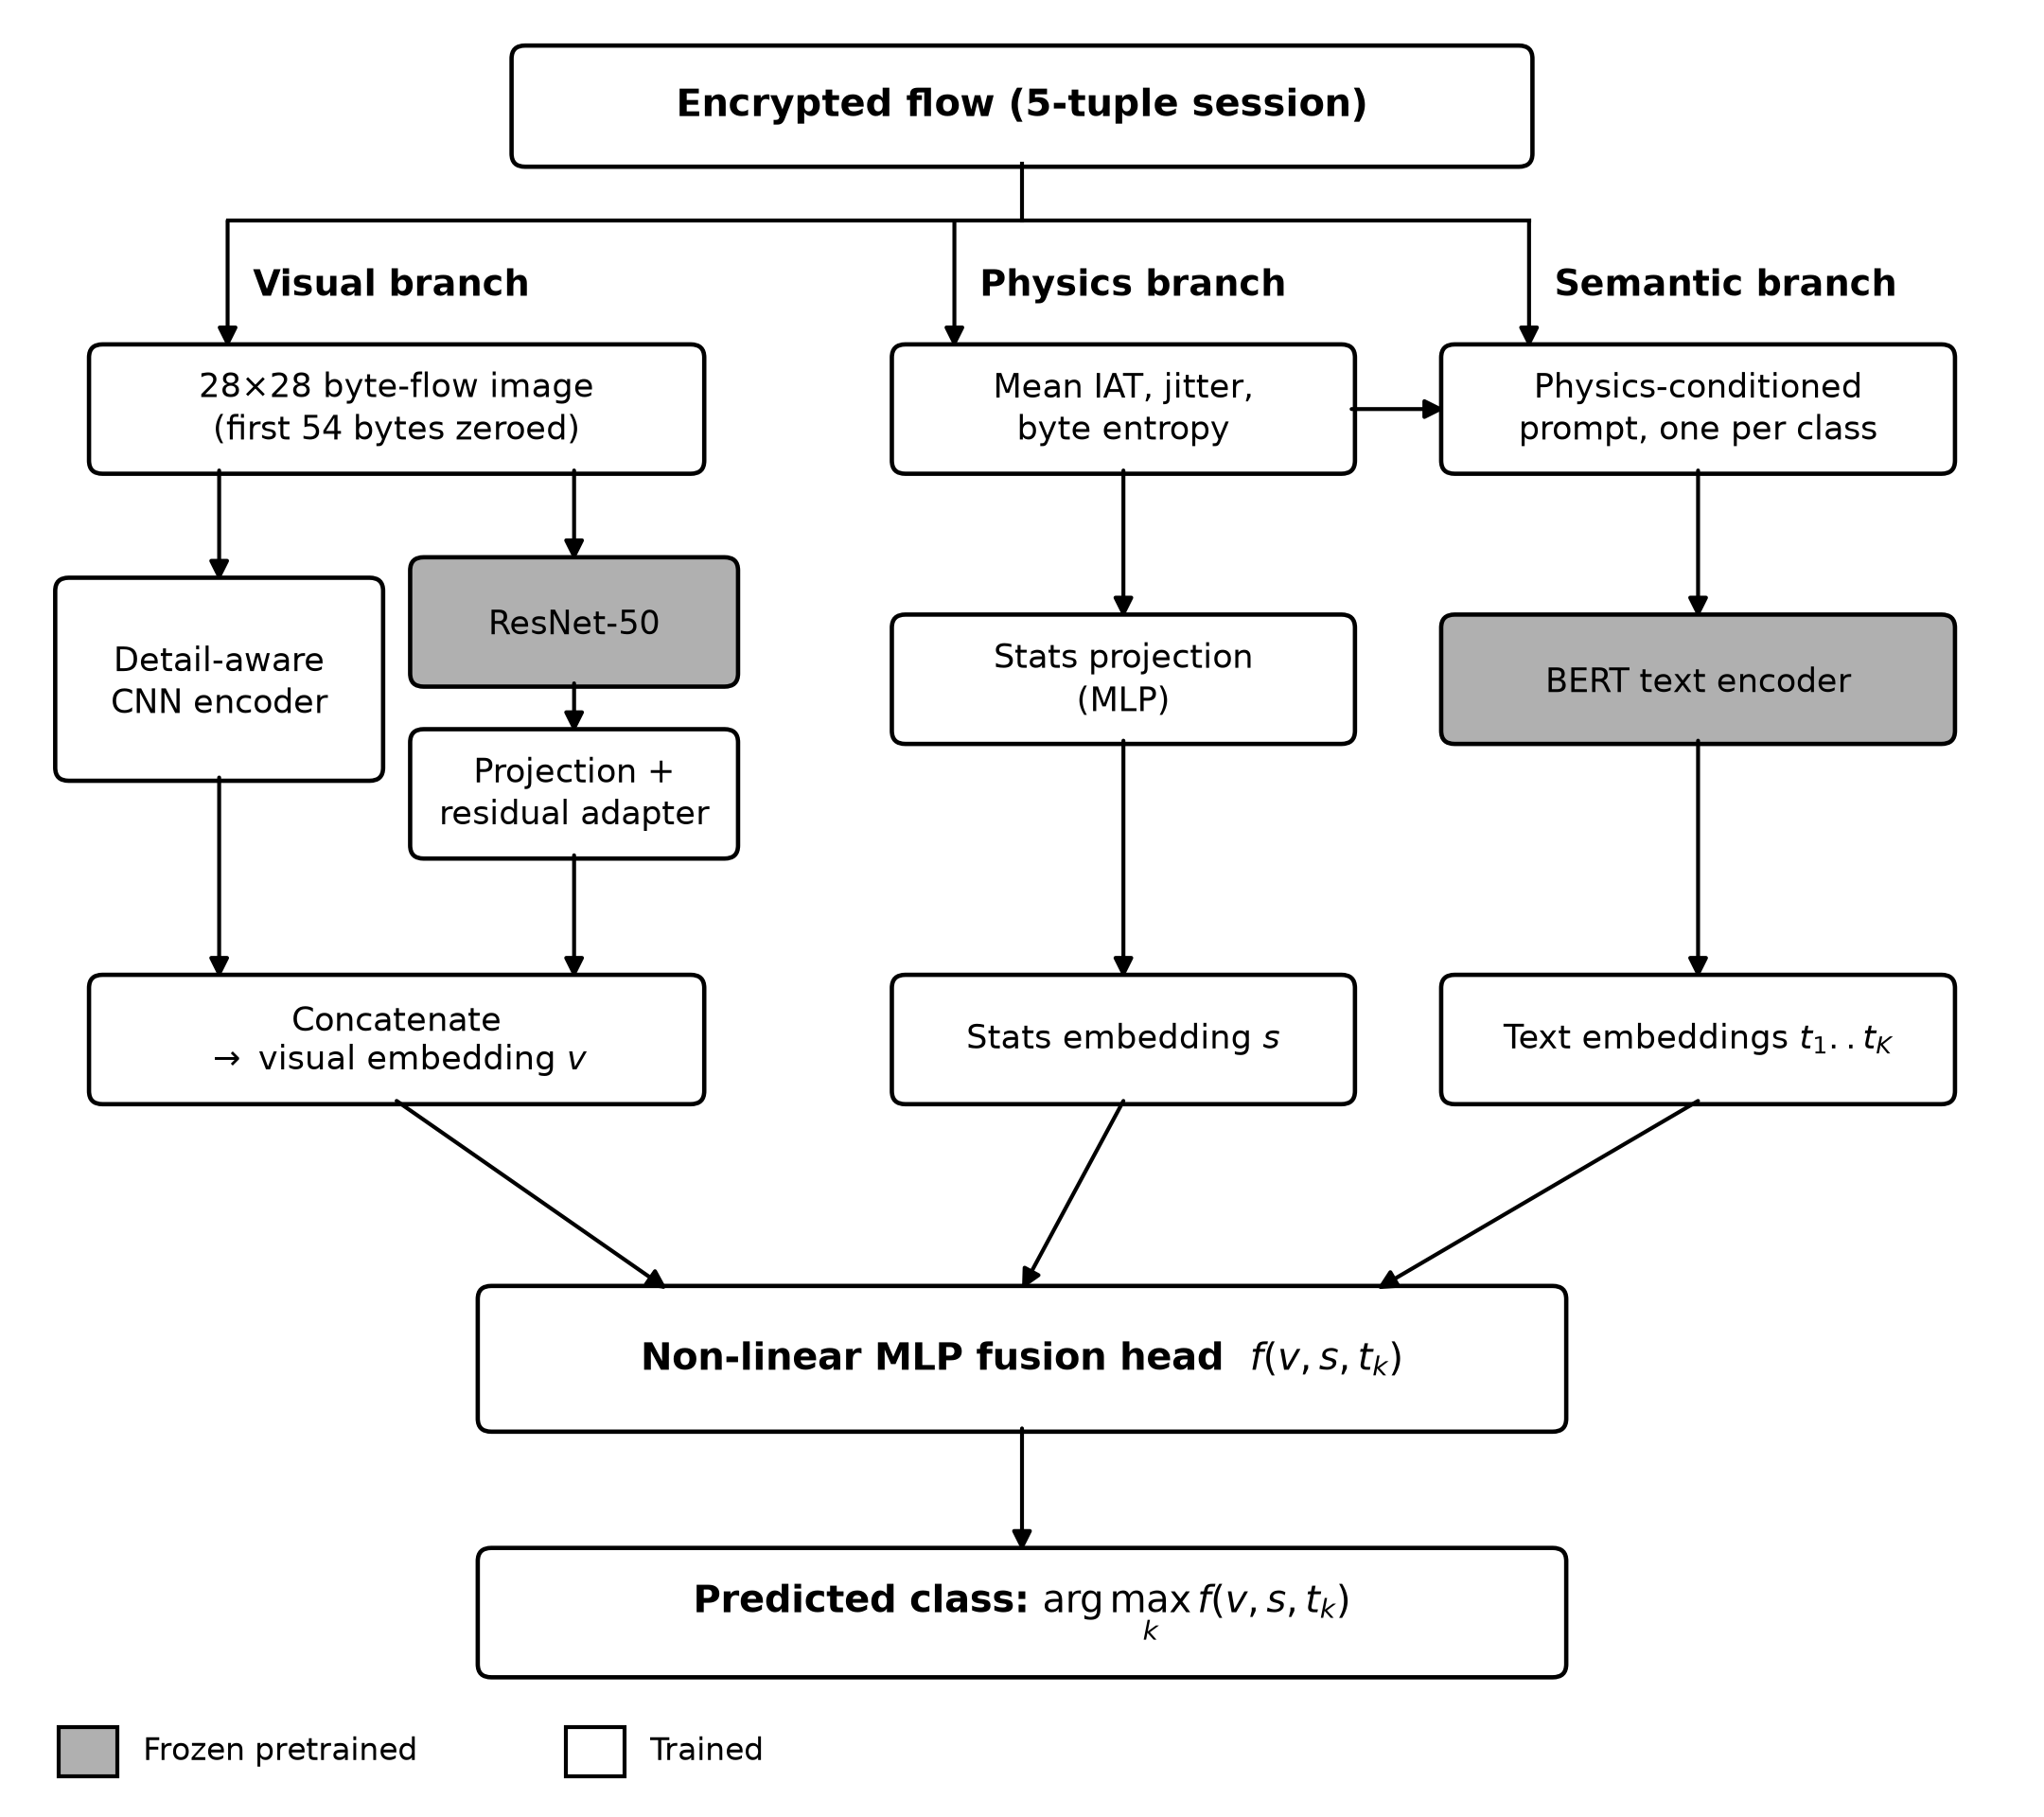
\includegraphics[width=\columnwidth]{architecture_bw.png}
\caption{Tri-modal OptimizedTrafficCLIP architecture. Grey blocks are frozen pretrained modules; white blocks are trained. The detail-aware encoder and the ResNet-50 path run in parallel and are concatenated.}
\label{fig:arch}
\end{figure}

\subsection{Visual Branch}
The first 784 bytes of each flow are reshaped into a $28 \times 28$ grayscale image, with the first 54 header bytes zeroed to remove trivially identifying fields. A trainable detail-aware convolutional encoder is combined with a semantics-aware branch built on a pretrained ResNet-50 backbone \cite{resnet}, adapted from three-channel to single-channel input and kept frozen. A lightweight traffic adapter and a residual connection combine the two sub-branches into a single visual embedding.

\subsection{Physics Branch}
Three session-level statistics, mean inter-arrival time, jitter, and byte entropy, are computed per flow and projected through a trainable stats projection head into a stats embedding. These same three statistics also condition the dynamic prompt consumed by the semantic branch.

\subsection{Semantic Branch}
Rather than a single static prompt per class name, each candidate class is rendered as a short natural-language description conditioned on the sample's own physics statistics. The resulting text is encoded by a frozen pretrained BERT model \cite{bert}, and the $K$ candidate embeddings, one per class, are scored against the fused vision-and-stats representation at inference time.

\subsection{Fusion and Training Objective}
A non-linear multilayer perceptron fusion head combines the visual, stats, and text embeddings and produces a class score, replacing the cosine-similarity classifier of the base TrafficCLIP design. The network is trained with a joint objective combining cross-entropy loss and a supervised contrastive loss term \cite{supcon}, weighted by a coefficient $\alpha$.

\section{Methodology}\label{sec:method}

\subsection{Audit Procedure Overview}\label{sec:framework}
The study follows a five-stage procedure. Each stage answers one question that the previous stages leave open, and each can be reused for auditing other released traffic classifiers. Table~\ref{tab:framework} lists the stages and where each is carried out in this paper.

\begin{table}[t]
\caption{Five-Stage Audit Procedure}
\label{tab:framework}
\centering
\renewcommand{\arraystretch}{1.2}
\begin{tabular}{|c|p{3.0cm}|p{3.6cm}|}
\hline
\textbf{Stage} & \textbf{Question} & \textbf{Instantiation here} \\
\hline
S1 & Does the released code implement the stated protocol? & Line-by-line audit; six defects (Table~\ref{tab:defects}) \\
\hline
S2 & What does the released code score once corrected? & In-place fixes, manuscript's own protocol, 5 seeds (Track B) \\
\hline
S3 & Is a remaining gap architectural or implementation-specific? & Clean-room bi-modal and tri-modal rebuilds (Tracks A, A-Full) \\
\hline
S4 & How hard is the task, and does the finding transfer? & Four external baselines; three additional datasets (Track C) \\
\hline
S5 & Where does the residual error come from? & Per-class and confusable-pair analysis, feature probe \\
\hline
\end{tabular}
\end{table}

S1 separates defects in the code from properties of the design. S2 measures what the released artifact actually achieves after correction, using the authors' own protocol so that the comparison with their reported table is like for like. S3 is the step most reproducibility studies omit: if the corrected release still falls short of a reference, only an implementation built without reference to the released code can tell whether the architecture or the implementation is responsible. S4 fixes the scale against which every other number is read, since a gain on a benchmark that unrelated models already saturate carries little information. S5 attributes the error that survives all corrections, so that the remaining gap is explained rather than left as an open discrepancy. Every stage shares one data split, verified identical across implementations by an automated test, and reports multi-seed statistics.


\subsection{Dataset and Split}\label{sec:data}
All experiments use USTC-TFC2016 \cite{ustc}, preprocessed identically across every track compared in this paper: flows are keyed by 5-tuple, the first 784 bytes are reshaped into a $28 \times 28$ grayscale image, and the first 54 header bytes are zeroed. Both a 10-class balanced subset at 900 samples per class and a 20-class extension are evaluated. All tracks use the same stratified 70/15/15 train, validation, and test partition at a fixed seed. An automated test asserts directly that the split indices generated independently by each implementation are identical for the same input archive, so the comparisons reported below are not an artifact of differing test sets.

\subsection{Defect Audit of the Released Implementation}
The released OptimizedTrafficCLIP repository was executed as documented and inspected line by line. Table~\ref{tab:defects} summarizes six defects found in its training and evaluation pipeline. All six were corrected in place, without altering the model architecture itself. Two further unrelated bugs were found and fixed while exercising the corrected pipeline against real data: the number of output classes was derived from the full 20-class taxonomy rather than from the loaded archive's actual label count, and the default experiment-tracking serialization path crashed at the end of every run.

\begin{table}[t]
\caption{Defects Identified in the Released Implementation}
\label{tab:defects}
\centering
\renewcommand{\arraystretch}{1.25}
\begin{tabular}{|c|p{3.1cm}|p{3.3cm}|}
\hline
\textbf{\#} & \textbf{Defect} & \textbf{Effect} \\
\hline
1 & Contrastive-loss weight $\alpha$ not exposed as a constructor argument & Manuscript's stated configuration unreachable through the documented API \\
\hline
2 & Evaluation forward pass embeds the ground-truth class name in the dynamic prompt & Evaluation-time label leakage that inflates the reported score \\
\hline
3 & Benchmark script regenerates the train and test split at a shifted seed on each repeated pass & Split leakage across repeated evaluation passes \\
\hline
4 & Hypothesis-testing validation loop processes one sample at a time and reads an unresolved class-name variable instead of the resolved list & Silent incorrectness in the dynamic-prompt evaluation path \\
\hline
5 & Training data loader built with shuffling disabled & Frozen batch composition degrades the contrastive loss term \\
\hline
6 & Frozen backbone submodules not forced into evaluation mode during training & Dropout remains active and batch-normalization statistics keep drifting despite frozen weights \\
\hline
\end{tabular}
\end{table}

\subsection{Honest Re-Evaluation Protocol}
After applying all six corrections, the manuscript's own hypothesis-testing evaluation protocol was re-executed at the manuscript's own reported seed, for every configuration the manuscript reports, allowing a direct comparison against its published table for the equivalent configurations.

\subsection{Independent Bi-Modal Reimplementation (Track A)}
A second implementation of the underlying TrafficCLIP architecture was built independently from the published specification, without consulting the released OptimizedTrafficCLIP code, so that no implementation choice of the release could propagate into the reference point.

\subsection{Independent Tri-Modal Reimplementation (Track A-Full)}
A further independent implementation extends Track A with OptimizedTrafficCLIP's two distinguishing components, the physics-statistics branch and physics-conditioned dynamic prompting, fused through a non-linear head. This implementation avoids Defects 1, 2, 3, 4, and 6 of Table~\ref{tab:defects} by construction: the data split is fixed once per dataset rather than regenerated per run, frozen submodules are pinned to evaluation mode inside the model's own training routine, and training uses the same batched multi-candidate hypothesis computation used at test time, so the model is never given the sample's true-label prompt as a training input.

Evaluating $K$ candidate prompts through a live text encoder at every training step does not scale; it was measured at approximately 7.5 seconds per step at $K=20$. Because every sample's physics statistics are fixed for a given run, its $K$ dynamic prompt strings and their text embeddings are fixed as well, so they are precomputed once into an $(N, K, 768)$ cache. An equivalence test asserts that cached and live hypothesis logits agree exactly, which gates every Track A-Full number reported here.

\subsection{Independent Baselines (Track C)}\label{sec:mc}
Four additional models were implemented from scratch and trained on the identical data and test split described in Section~\ref{sec:data}: FlowPic \cite{flowpic}, FS-Net \cite{fsnet}, a 1D convolutional network over the raw byte sequence, and a small Transformer encoder over the same sequence chunked into tokens. All four consume the same $28 \times 28$ byte-flow image (equivalently, the 784-byte sequence) used by Tracks A and A-Full. For FlowPic and FS-Net specifically, this substitutes for their own originally published input representations, FlowPic's packet-size/inter-arrival-time histogram and FS-Net's signed per-packet-length sequence. That substitution was closed in a follow-up run: raw packet captures were re-acquired, and both baselines were re-trained on their own published representations, extracted directly from the same underlying flows (Section~\ref{sec:rcorig}). No published FlowPic or FS-Net evaluation exists on USTC-TFC2016 itself, so the comparison is necessarily each baseline's own representation against the byte-image substitution on the same data, not a same-dataset published-versus-reproduced comparison.

\subsection{Cross-Dataset Datasets}\label{sec:mcross}
To test whether Track A and Track A-Full's parity result is specific to USTC-TFC2016 or generalizes, both tracks and all four Track C baselines were re-run, unmodified beyond the number of output classes, on three additional, independently sourced datasets spanning a different application domain, network generation, and traffic-collection methodology each:

\begin{itemize}
\item \textbf{ISCXVPN2016} \cite{iscxvpn}: a 3.1\,GB "01" split of the public VPN/non-VPN traffic corpus, re-labeled into a 5-class traffic-type taxonomy (Chat, Email, File Transfer, P2P, VoIP/Video) by folding VPN and non-VPN captures of the same type into one class, so the task remains traffic-type classification rather than VPN-detection. The split is naturally imbalanced (File Transfer: 127 samples, P2P: 487, against 900 each for the three larger classes), reported as-is rather than rebalanced. 2,914 samples total.
\item \textbf{5G Traffic Capture Dataset} \cite{g5traffic}: the 2.3\,GB inference split of a University of Juiz de Fora 5G-core dataset, four continuous packet captures labeled by traffic type (eMBB video streaming, URLLC live streaming, mMTC low-rate UDP telemetry). Each capture is a single sustained session on one flow 5-tuple, so a 60-second idle-timeout is applied when segmenting flows (Section~\ref{sec:data}'s own protocol uses no timeout, since USTC-TFC2016's captures do not need one); mMTC remains the smallest class at 59 samples, since the corpus itself ships only two mMTC captures, one of them a perfectly constant-rate synthetic generator with no idle gaps to split on. 472 samples total.
\item \textbf{IoT-23} \cite{iot23}: a hand-selected, 2.5\,GB, 9-class subset (3 real, non-simulated benign IoT devices; 6 malware family captures) of the Stratosphere Laboratory's IoT malware/benign corpus, chosen to fit a small-dataset budget from a 21\,GB full release. The same 60-second flow-idle-timeout is applied, which matters for one class specifically: a sustained Mirai DDoS-flood capture yields only 20 usable flow samples without a timeout against 229 with it, since a flood targeting one victim IP is otherwise a single, arbitrarily long same-5-tuple flow. 6,340 samples total, imbalanced by capture availability (Mirai: 229, Somfy Doorlock: 258, Philips Hue: 453, all other classes at the 900-sample cap).
\end{itemize}

All three datasets use the identical preprocessing, split protocol, and evaluation code as Section~\ref{sec:data}; only the source \texttt{.npz} archive and class count change.

\subsection{An Additional Divergence: Visual Stem Initialization}\label{sec:mstem}
Beyond the six defects of Table~\ref{tab:defects}, the release diverges from the pretrained backbone's intended use in a way that the independent tracks handle differently. ResNet-50's first convolutional layer is a $(64, 3, 7, 7)$ kernel trained for three-channel input. The release replaces it outright with a freshly initialized single-channel \texttt{Conv2d(1, 64, 7, 7)} and then freezes it, so the frozen backbone receives an untrained random first-layer projection. Tracks A and A-Full instead adapt the pretrained kernel to single-channel input by summing its weights across the input-channel dimension, which is equivalent to replicating a grayscale image across the three original channels. Because this was the leading prior hypothesis for the release's underperformance, an ablation variant reinstalls the release's version verbatim inside each otherwise correct codebase, with every other component held fixed, to isolate its individual contribution.

\section{Experimental Setup}\label{sec:setup}

All training runs were executed on a single Apple M4 GPU using the Metal Performance Shaders backend. Tracks A and A-Full were each trained for 200 epochs per configuration and averaged over 3 independent seeds. Track C baselines were trained for an equivalent budget and averaged over 5 independent seeds. Track B's honest re-evaluation was likewise re-run across 5 independent seeds (62--66) for all six configurations, matching the manuscript's own protocol at each seed. Pairwise Wilcoxon signed-rank tests with Bonferroni correction were computed across all 15 configuration pairs; at $n=5$ seeds the exact two-sided test cannot fall below $p=0.0625$ regardless of effect size, so a null result at this sample size reflects that structural floor rather than a finding of no difference, and is reported as such rather than suppressed. Accuracy and Macro F1 are reported as the primary metrics throughout, since the class distribution is only approximately balanced at the 20-class setting.

\section{Results}\label{sec:results}

\subsection{Tracks A and A-Full: Independent Reimplementations}\label{sec:rafull}
Table~\ref{tab:a} reports both independent reimplementations under the identical protocol. The tri-modal Track A-Full matches the bi-modal Track A to within 0.1 point at both class counts, so the added physics and dynamic-prompt modalities neither help nor hurt on this dataset once implemented correctly. Accuracy and Macro F1 coincide to within 0.01 point because the test partitions are near-balanced, so only accuracy is shown.

\begin{table}[t]
\caption{Tracks A and A-Full on USTC-TFC2016 (Percent Accuracy, Mean $\pm$ SD, 3 Seeds)}
\label{tab:a}
\centering
\renewcommand{\arraystretch}{1.2}
\begin{tabular}{|l|c|c|}
\hline
\textbf{Configuration} & \textbf{Track A (bi-modal)} & \textbf{Track A-Full (tri-modal)} \\
\hline
10-class & 99.75 $\pm$ 0.09 & 99.68 $\pm$ 0.07 \\
\hline
20-class & 96.64 $\pm$ 0.23 & 96.63 $\pm$ 0.09 \\
\hline
\end{tabular}
\end{table}

\textbf{Visual stem ablation.} Reinstalling the release's untrained, frozen single-channel stem (Section~\ref{sec:mstem}) inside each otherwise correct codebase leaves 20-class accuracy unchanged within seed variance: 96.68\% $\pm$ 0.14 against 96.64\% for Track A, and 96.80\% $\pm$ 0.20 against 96.63\% for Track A-Full. This divergence therefore does not explain the release's shortfall.

\subsection{Track B: Honest Re-Evaluation of the Released Code}
Table~\ref{tab:b} compares the manuscript's own reported values for all six of its configurations under its stated hypothesis-testing protocol against the same configurations re-measured, across 5 seeds each, after the six defects of Table~\ref{tab:defects} are corrected. The four configurations that rely on a static hard prompt (V1, V2, V3, V5) collapse once the label-leaking evaluation path is repaired, which is the behavior a genuine leak predicts. The two configurations that use the physics-conditioned dynamic prompt (V4 and Full) instead improve: V4 rises by 7.6 points of Macro F1 (5-seed mean) and Full by 8.7 points. The manuscript's separately reported headline figure of 87.54\% originates from a distinct forward-pass evaluation path whose text input carries the ground-truth label, and is not reproduced under the corrected protocol. A pairwise Wilcoxon signed-rank test with Bonferroni correction across all six configurations found no Bonferroni-significant pairs, but as noted in Section~\ref{sec:setup} this null result reflects the $n=5$ floor ($p \geq 0.0625$) rather than genuine equivalence between the dynamic- and static-prompt configurations. A paired $t$-test with the same correction separates V4 and Full from every static-prompt configuration ($p<0.001$), while V4 and Full do not differ from each other ($p=0.93$).

\textbf{Variance across seeds.} The dynamic-prompt configurations are also the more stable ones. V4 has the smallest seed-to-seed spread of all six configurations (SD 0.87, 95\% $t$-interval $\pm$1.08 points, range 85.27 to 87.13), and Full's SD of 2.15 ($\pm$2.67) is below that of every static-prompt configuration except V1 (1.52). Relative to the mean, the gap is wider: the coefficient of variation is 1.0\% for V4 and 2.4\% for Full, against 5.1\%, 20.4\%, 12.4\%, and 8.0\% for V1, V2, V3, and V5. The static-prompt configurations, V2 and V3 in particular, swing by 11 to 16 points of Macro F1 between seeds (V2 from 23.03 to 39.45), so a single-seed measurement of them could land almost anywhere in that range. With five seeds per configuration this comparison is descriptive; it is not backed by a formal test for equality of variances.

\begin{table}[t]
\caption{Track B, Manuscript-Reported Against Defect-Corrected Measurement Under the Manuscript's Own Protocol (Percent Macro F1, Mean $\pm$ SD, 5 Seeds)}
\label{tab:b}
\centering
\renewcommand{\arraystretch}{1.2}
\begin{tabular}{|l|p{2.1cm}|c|c|}
\hline
\textbf{Var.} & \textbf{Configuration} & \textbf{Reported} & \textbf{Corrected} \\
\hline
V1 & Original, no stats & 62.21 & 29.54 $\pm$ 1.52 \\
\hline
V2 & Original, with stats & 59.05 & 31.54 $\pm$ 6.43 \\
\hline
V3 & Optimized, hard prompt & 63.10 & 39.66 $\pm$ 4.90 \\
\hline
V4 & Optimized, dynamic prompt & 78.57 & \textbf{86.19 $\pm$ 0.87} \\
\hline
V5 & Optimized, hard prompt, stats & 67.01 & 43.83 $\pm$ 3.50 \\
\hline
Full & Optimized, dynamic prompt, stats & 79.63 & \textbf{88.29 $\pm$ 2.15} \\
\hline
\end{tabular}
\end{table}

\subsection{Track C: Independent Baselines}\label{sec:rcorig}
Table~\ref{tab:c} reports all four Track C models trained from scratch on the identical data and split. On the shared byte-image representation every model exceeds 99\% accuracy at 10 classes and 93\% at 20, matching Tracks A and A-Full with four architecturally unrelated families. FlowPic and FS-Net were additionally re-trained on their own originally published input representations, extracted from re-acquired raw packet captures for the identical flows: FlowPic's packet-size/inter-arrival-time histogram and FS-Net's signed per-packet-length sequence. Both score measurably lower on their own representation (FlowPic: 18.7 points lower at 10 classes, 29.2 at 20; FS-Net: 7.8 and 14.5), confirming the direction that Section~\ref{sec:mc}'s substitution caveat predicted. Neither original paper evaluates on USTC-TFC2016, so no same-dataset published number exists to compare either representation against.

\begin{table}[t]
\caption{Track C Baselines on USTC-TFC2016 (Percent Accuracy, Mean $\pm$ SD, 5 Seeds)}
\label{tab:c}
\centering
\renewcommand{\arraystretch}{1.2}
\setlength{\tabcolsep}{3pt}
\begin{tabular}{|l|c|c|c|c|}
\hline
 & \multicolumn{2}{c|}{\textbf{Byte image}} & \multicolumn{2}{c|}{\textbf{Own representation}} \\
\cline{2-5}
\textbf{Model} & \textbf{10-class} & \textbf{20-class} & \textbf{10-class} & \textbf{20-class} \\
\hline
FlowPic & 99.39 $\pm$ 0.06 & 93.87 $\pm$ 0.35 & 80.71 $\pm$ 0.06 & 64.63 $\pm$ 0.57 \\
\hline
FS-Net & 99.45 $\pm$ 0.18 & 95.50 $\pm$ 0.29 & 91.67 $\pm$ 0.39 & 80.96 $\pm$ 0.95 \\
\hline
1D-CNN & 99.63 $\pm$ 0.10 & 96.21 $\pm$ 0.22 & -- & -- \\
\hline
Transformer & 99.50 $\pm$ 0.14 & 95.17 $\pm$ 0.41 & -- & -- \\
\hline
\end{tabular}
\end{table}

\subsection{Cross-Dataset Generalization}\label{sec:rcross}
Table~\ref{tab:cross} reports Tracks A and A-Full and all four Track C baselines, unmodified beyond output class count, on the three additional datasets of Section~\ref{sec:mcross}. Macro F1 is shown because these datasets are imbalanced. On every dataset the two independent tracks remain within one standard deviation of each other, replicating the USTC-TFC2016 parity finding of Section~\ref{sec:rafull} on a VPN traffic-type task, a 5G network-slice task, and an IoT device/malware-family task. Every model exceeds 85\% Macro F1 on every dataset, and the ranking among the baselines is not consistent across datasets (FS-Net leads on 5G, 1D-CNN on ISCXVPN2016 and IoT-23), so no single architecture is uniformly superior across traffic domains. The Transformer's wide spread on ISCXVPN2016 (5.14 points) is the largest in the table and most likely reflects its instability on a small, imbalanced training set, since the same model is within 1.1 points of the 1D-CNN at 20 classes on USTC-TFC2016.

\begin{table}[t]
\caption{Cross-Dataset Generalization (Percent Macro F1, Mean $\pm$ SD; 3 Seeds for Tracks A and A-Full, 5 for Track C)}
\label{tab:cross}
\centering
\renewcommand{\arraystretch}{1.2}
\setlength{\tabcolsep}{4pt}
\begin{tabular}{|l|c|c|c|}
\hline
\textbf{Model} & \textbf{ISCXVPN2016} & \textbf{5G} & \textbf{IoT-23} \\
\hline
Track A & 92.06 $\pm$ 0.96 & 98.20 $\pm$ 1.35 & 98.23 $\pm$ 0.27 \\
\hline
Track A-Full & 91.47 $\pm$ 0.96 & 98.91 $\pm$ 0.89 & 98.67 $\pm$ 0.32 \\
\hline
FlowPic & 90.88 $\pm$ 0.58 & 97.81 $\pm$ 0.00 & 97.99 $\pm$ 0.13 \\
\hline
FS-Net & 89.54 $\pm$ 1.01 & 98.24 $\pm$ 0.90 & 97.96 $\pm$ 0.38 \\
\hline
1D-CNN & 92.86 $\pm$ 0.65 & 96.91 $\pm$ 1.10 & 98.26 $\pm$ 0.18 \\
\hline
Transformer & 85.00 $\pm$ 5.14 & 95.88 $\pm$ 1.58 & 97.40 $\pm$ 0.38 \\
\hline
\end{tabular}
\end{table}

\subsection{Anatomy of a Confusable Pair}\label{sec:anatomy}
Broken down by class, Track A-Full's 20-class result is uneven. Nine classes are classified perfectly on every seed, eighteen of twenty are at or above 95\%, and the two exceptions are the botnet families Virut (68.40\%) and Neris (78.02\%). Summed over three seeds, 207 of the model's 273 test errors (75.8\%) are confusions between these two classes, from 70.5\% to 82.4\% on individual seeds.

\textbf{Why the physics-statistics branch cannot separate them.} Both classes contain 900 flows in the dataset. Their per-flow statistics, computed directly from the test split and independent of any model, have nearly identical medians: inter-arrival time 1793\,ms against 1783\,ms, jitter 2399\,ms against 2396\,ms, and byte entropy 4.94 against 4.93. The means differ widely (inter-arrival time 181{,}107\,ms against 17{,}976\,ms), but only because of a small number of extreme outliers; the bulk of the two distributions coincides. Since the statistics branch and the dynamic prompt both read exactly these three values, the tri-modal model receives almost no information from them that distinguishes the typical Virut flow from the typical Neris flow, and must rely on the byte image. Once a flow is assigned to one of the two classes, A-Full separates them correctly 74.1\% of the time (593 of 800 decisions).

\textbf{Do additional features help?} To test whether other flow properties carry the missing signal, seven features absent from the three-value statistics vector were computed from the raw captures of the same 900 flows per class: packet-size mean, standard deviation, and skewness; burst count and mean burst size at a 1\,s idle gap; and byte entropy over only the first 200 and only the last 200 bytes of each flow. A two-sample Welch $t$-test was applied to each. The most informative features concern where in the flow entropy is measured rather than its overall level: last-200-byte entropy differs strongly between the classes ($t=9.27$, $p=5\times10^{-20}$), as does first-200-byte entropy ($t=5.67$, $p<10^{-7}$), while whole-flow entropy does not. Packet-size mean ($p=0.003$) and skewness ($p=0.006$) differ moderately; packet-size spread and burst statistics do not differ significantly ($p\geq0.08$). A logistic regression on the seven features alone separates the pair with 61.4\% $\pm$ 4.9\% accuracy under 5-fold cross-validation, against a 50\% chance level. This is real but modest signal, and on its own it is weaker than the 74.1\% that A-Full already achieves from the byte image. Whether the extra features are complementary to the image branch, and would therefore reduce the pair's error when added to the model, requires retraining the tri-modal model with an extended statistics vector for all twenty classes; this was not performed and is left to future work.

\textbf{Implications for deployment.} For eighteen of twenty classes the tri-modal model is at or near ceiling, and an operator can rely on its per-class output directly. For Virut and Neris, roughly one flow in four is attributed to the wrong family. Both are botnets, so a deployment that needs only to flag botnet traffic can merge the two into one alert class with little loss. One that must attribute a flow to the correct family should treat the pair as a single ambiguous group and resolve it with a second-stage decision or with evidence beyond a single flow, such as host-level behavior across many flows. An aggregate accuracy of 96.6\% hides this failure mode entirely, which is why per-class reporting is among the recommendations of Section~\ref{sec:recs}.

\section{Discussion}\label{sec:discussion}

The results in Section~\ref{sec:results} support a single central conclusion: OptimizedTrafficCLIP's measured accuracy gap against a defect-free reference is a property of the released implementation, not of the tri-modal architecture it implements. Track A-Full, an independent rebuild of the identical tri-modal design, reaches 99.68\% accuracy on the 10-class benchmark, essentially matching Track A's simpler bi-modal design and 11.6 percentage points above Track B's corrected 5-seed mean of 88.13\% for the same architecture on the same task.

The visual stem ablation of Section~\ref{sec:rafull} further shows that the gap cannot be attributed to the single divergence that was most suspected in advance. Replacing the adapted pretrained convolution kernel with an untrained frozen one effectively feeds the frozen backbone a random first-layer projection, yet isolated inside an otherwise correct codebase it costs approximately nothing in either independent track. The most likely explanation is that the trainable detail-aware branch and the trainable adapter and fusion parameters have enough capacity to compensate for a randomized first convolutional layer on a dataset this separable.

Track C's baselines contextualize the finding further. Four architecturally unrelated models, a two-dimensional convolutional network over the byte image, a bidirectional recurrent encoder, a 1D convolutional network, and a small Transformer, all exceed 99\% accuracy on the 10-class benchmark when trained from scratch on the same data. The 10-class USTC-TFC2016 task is therefore close to solved by several different architectural families, which is the appropriate context for reading Track B's corrected 88.13\% $\pm$ 2.12\% accuracy: it reflects this specific implementation's defect profile and training budget on this task, and is not evidence that the task itself is difficult.

Cross-dataset generalization (Section~\ref{sec:rcross}) extends the central finding beyond a single corpus. Tracks A and A-Full remain statistically indistinguishable on ISCXVPN2016 (a VPN traffic-type task), a 5G traffic dataset (a network-slice task), and IoT-23 (an IoT device/malware-family task), three datasets that differ from USTC-TFC2016 and from each other in application domain, network generation, and collection methodology. The tri-modal design's parity with its simpler bi-modal counterpart is therefore not an artifact of one dataset's specific separability; it replicates on four independent datasets spanning four different classification problems. Track C's four baselines generalize similarly, each exceeding 85\% Macro F1 on every dataset with no single baseline uniformly ahead across all three, which argues against reading Track B's gap as a general property of frozen-backbone or CLIP-style approaches on this class of task, since three unrelated architectural families make the same problems look easy regardless of source dataset.

Table~\ref{tab:b} shows that OptimizedTrafficCLIP's own central contribution, physics-conditioned dynamic prompting, is a real and reproducible mechanism. Under the manuscript's own protocol, correcting the six identified defects raises the Full configuration from a single-run 79.63\% to an 88.29\% $\pm$ 2.15\% 5-seed mean Macro F1 rather than lowering it, and only the two dynamic-prompt configurations clear 80\% once the leak is repaired. What does not reproduce is the separately reported 87.54\% headline figure, which this audit traces to a distinct evaluation-path defect rather than to the architectural contribution itself.

\subsection{Why the Label Leak Inflated the Reported Score}
In OptimizedTrafficCLIP the text branch reads a sentence built from a class name and the flow's physics statistics. At training time the true class name is a legitimate input, because the contrastive objective needs a positive pair. At evaluation time it is not, because the class name is exactly what the model must predict. The released evaluation path that produced the 87.54\% figure built each sample's prompt from that sample's own ground-truth class and took the argmax of a single forward pass. The correct class name was therefore present in the input the fusion head read before making its prediction, and the head could recover the label from the text branch without using the visual or statistical evidence at all. The label-free alternative, which the manuscript's own hypothesis-testing protocol specifies, scores all $K$ candidate prompts and selects the best match; this is the protocol under which every corrected number in this paper is measured. The pattern in Table~\ref{tab:b} is what this mechanism predicts. Configurations whose text input carries little besides the class name (V1, V2, V3, V5) lose between 23 and 33 points once the label is removed, because that name was most of what they relied on. The dynamic-prompt configurations (V4, Full), whose prompts also carry per-sample statistics, do not collapse. In the taxonomy of Kapoor and Narayanan \cite{kapoor2023} this is leakage from the target into the evaluation-time input. It is easy to miss because the same prompt-construction code is correct in training and wrong in evaluation.

\subsection{Why Independent Verification Matters in This Field}
Three results of this study could not have come from re-running the released code alone. First, the corrected release scores 88.13\% accuracy at 10 classes, yet a clean-room build of the same architecture reaches 99.7\% on the same task. Running only the release would wrongly suggest that the tri-modal design is weak. Second, the byte-image substitution for FlowPic and FS-Net inflates their accuracy by 7.8 to 29.2 points (Table~\ref{tab:c}), so an input representation that is left unstated can move a baseline by more than the gap between competing methods. Third, the residual error of a correct implementation concentrates in one class pair (Section~\ref{sec:anatomy}), which a single aggregate number conceals. Each of these can be caught only by building something independently and comparing. Recent evidence points the same way: encrypted-traffic classifiers validated on controlled datasets lose accuracy on production traffic \cite{malekghaini2023}, and near-perfect detectors trained on one public dataset may not transfer to separately generated traffic \cite{catillo2022}. Independent verification is therefore not a formality in this field; it is how architectural claims are separated from pipeline artifacts.

\subsection{What a Saturated Benchmark Means for the Field}
Six models of five kinds (CLIP-style bi-modal and tri-modal models, 2D and 1D convolutional networks, a recurrent encoder, and a Transformer) all exceed 99\% on the 10-class USTC-TFC2016 task and lie within 2.8 points of each other at 20 classes (93.9\% to 96.6\%). On such a benchmark a new architecture cannot show a meaningful improvement in accuracy, and differences of a few tenths of a point sit inside seed-to-seed variance. Claims of novelty on USTC-TFC2016 should therefore rest on something other than headline accuracy: robustness to distribution shift, cost, interpretability, or performance on the hard residual pairs that a saturated aggregate hides. It also follows that a reported shortfall on this benchmark is more likely to indicate an implementation problem than a limitation of the architecture, which is exactly what this study found.

\section{Limitations}\label{sec:limitations}

The following limitations bound the conclusions of this study.

\begin{itemize}
\item \textbf{Statistical power of the Track B significance test.} Track B is averaged over five seeds. At $n=5$ the exact two-sided Wilcoxon signed-rank test cannot fall below $p=0.0625$, so the pairwise Wilcoxon test has no power to reject at any Bonferroni-corrected level; the comparison rests on the paired $t$-test, which assumes approximately normal seed-to-seed differences.
\item \textbf{Unequal seed counts.} Tracks A and A-Full use three seeds and Tracks B and C use five, set by the per-run compute cost of each track on a single GPU.
\item \textbf{Track B is evaluated on USTC-TFC2016 only.} The released code is specific to the original 10- and 20-class taxonomy, so the cross-dataset extension covers Tracks A, A-Full, and C but not B.
\item \textbf{Partly constrained baselines.} FlowPic and FS-Net were re-trained on their own published representations, but the 1D-CNN and the Transformer are generic architectures rather than reimplementations of specific published models, and all baselines use one training budget without per-dataset tuning.
\item \textbf{Small, imbalanced additional datasets.} The 5G dataset's mMTC class has 59 samples from two source captures and IoT-23's Mirai class has 229, reported as collected rather than rebalanced; the 5G Transformer cell shows a correspondingly wide seed-to-seed spread.
\item \textbf{Residual-error analysis is limited to one pair.} The additional features of Section~\ref{sec:anatomy} were computed only for Virut and Neris and tested with a standalone classifier; a retrain of the tri-modal model with an extended statistics vector for all twenty classes was not performed, so whether those features would reduce the pair's error inside the model remains open.
\item \textbf{No adversarial or open-set evaluation.} Robustness to adversarially shaped packet timing or padding, and behavior on traffic classes unseen during training, were not tested.
\item \textbf{Single hardware platform.} All runs used one Apple M4 GPU with the Metal Performance Shaders backend; run-to-run numerical behavior on CUDA hardware was not checked.
\end{itemize}

\section{Recommendations for Reproducible Research in Encrypted Traffic Classification}\label{sec:recs}

Each defect in Table~\ref{tab:defects} and each correction in this study suggests a practice that would have prevented or exposed it. We group them by the stage of the research cycle at which they apply.

\subsection{Code Release}
\begin{enumerate}
\item \textbf{Release one evaluation path, and make it label-free by construction.} The headline figure and the corrected table came from different code paths. A single evaluation entry point whose inputs demonstrably exclude the target (Defect 2) removes this failure mode. A unit test that shuffles labels and checks that accuracy drops to chance is a cheap guard.
\item \textbf{Fix the data split once and assert it.} Persist the train, validation, and test indices, or derive them from a single fixed seed, and add a test that fails if two scripts produce different splits (Defect 3). Every comparison in this paper is gated on such a test.
\item \textbf{Pin framework modes explicitly.} Frozen submodules should be forced into evaluation mode inside the training loop, and data loaders should shuffle during training (Defects 5 and 6). Neither is visible in the reported numbers, so both should be tested directly.
\item \textbf{Expose every hyperparameter the paper reports.} A configuration named in the paper but unreachable through the released interface (Defect 1) cannot be reproduced as described.
\end{enumerate}

\subsection{Reporting}
\begin{enumerate}
\setcounter{enumi}{4}
\item \textbf{Report multi-seed statistics with the test's power stated.} Report a mean with a standard deviation or confidence interval over at least five seeds. If a significance test is used, state its minimum attainable $p$-value at the chosen sample size; at least ten paired seeds are needed before a Wilcoxon test can survive a Bonferroni correction over fifteen comparisons.
\item \textbf{State input representations exactly.} When a baseline is run on a representation other than its published one, say so and, where possible, report both, since the choice alone moved accuracy by up to 29 points here.
\item \textbf{Contextualize against saturated baselines.} Report at least one simple from-scratch baseline on the same split, so that readers can see how much of the benchmark is already solved.
\item \textbf{Report per-class results.} An aggregate of 96.6\% concealed a pair at 68\% and 78\%. Per-class accuracy and the confusion matrix should accompany every multi-class result.
\end{enumerate}

\subsection{Verification}
\begin{enumerate}
\setcounter{enumi}{8}
\item \textbf{Verify independently before publication.} A clean-room reimplementation from the paper's own description, by someone who has not read the released code, tests both the paper and the code at once. Where it disagrees with the release, the disagreement locates a defect.
\item \textbf{Test on at least one additional dataset.} A finding that holds on one benchmark may reflect that benchmark's separability; replication on independently collected data is inexpensive once the pipeline accepts an arbitrary class count.
\item \textbf{Publish a reproducibility checklist with the artifact.} A checklist in the style of the NeurIPS program \cite{pineau2021}, adapted to traffic data (capture source, flow segmentation and timeout, header masking, split procedure, seed list), lets reviewers check the points above without re-running the code.
\end{enumerate}

\section{Conclusion}

This paper reports an independent reproducibility study of OptimizedTrafficCLIP. A line-by-line audit of the released implementation identified six defects in its training and evaluation pipeline, one of which directly leaks the ground-truth label into the evaluation path. Correcting all six and re-running the manuscript's own evaluation protocol over five seeds raises the Full configuration from a single-run 79.63\% to 88.29\% Macro F1. The dynamic-prompting mechanism is therefore genuine, while the separately reported 87.54\% headline figure is not reproducible. Two independent reimplementations, one bi-modal and one tri-modal, reach 99.7\% accuracy on the 10-class benchmark, 11.6 points above the corrected release, which shows that the architecture is not the limiting factor. Four from-scratch baselines exceed 99\% on the 10-class task, so the benchmark is largely solved by several unrelated model families. The error that remains in a correct implementation is concentrated in a single pair of botnet families that the physics statistics cannot separate. The bi-modal and tri-modal parity result replicates on three independently sourced datasets covering VPN traffic type, 5G network slices, and IoT device and malware families.

The study's broader output is methodological: a five-stage audit procedure and eleven recommendations that, applied before publication, would have caught every defect reported here. Future work includes re-targeting the released code to the additional datasets so that its gap can be tested beyond USTC-TFC2016, retraining the tri-modal model with an extended statistics vector for all classes, evaluating open-set and adversarial robustness, and applying the same audit procedure to other released encrypted-traffic classifiers.

\section*{Code and Data Availability}
All code for the corrected release, both independent reimplementations, the four baselines, the dataset extraction scripts, and the per-seed result files underlying every table and figure in this paper are available in a public reproducibility package at \texttt{https://github.com/rrsd2769/traf{}ficCLIP}. The four datasets are publicly available from their original sources \cite{ustc,iscxvpn,g5traffic,iot23}.

\section*{Acknowledgment}

The authors thank Pramit De for the original OptimizedTrafficCLIP architecture and manuscript that this study reproduces, validates, and extends.

\begin{thebibliography}{00}
\bibitem{de2026otc} P. De, ``OptimizedTrafficCLIP: A tri-modal cross-modal framework for encrypted network traffic classification with physics-informed prompting and edge deployment,'' unpublished manuscript, 2026.
\bibitem{flowpic} T. Shapira and Y. Shavitt, ``FlowPic: A generic representation for encrypted traffic classification and applications identification,'' \emph{IEEE Trans. Netw. Serv. Manag.}, vol. 18, no. 2, pp. 1218--1232, 2021.
\bibitem{ustc} W. Wang, M. Zhu, X. Zeng, X. Ye, and Y. Sheng, ``Malware traffic classification using convolutional neural network for representation learning,'' in \emph{Proc. IEEE ICOIN}, 2017, pp. 712--717.
\bibitem{fsnet} C. Liu, L. He, G. Xiong, Z. Cao, and Z. Li, ``FS-Net: A flow sequence network for encrypted traffic classification,'' in \emph{Proc. IEEE INFOCOM}, 2019, pp. 1171--1179.
\bibitem{dong2025review} W. Dong, J. Yu, X. Lin, G. Gou, and G. Xiong, ``Deep learning and pre-training technology for encrypted traffic classification: A comprehensive review,'' \emph{Neurocomputing}, vol. 617, Art. no. 128444, 2025.
\bibitem{yang2025robust} L. Yang, L. Liu, J.-J. Huang, J. Shi, S. Fu, Y. Wang, and J. Su, ``Robustness matters: Pre-training can enhance the performance of encrypted traffic analysis,'' \emph{IEEE Trans. Inf. Forensics Security}, vol. 20, pp. 10588--10603, 2025.
\bibitem{zhao2026fewshot} L. Zhao, C. Wu, and A. Yu, ``When pre-training meets contrast learning: Few-shot encrypted traffic classification with novelty detection,'' \emph{IEEE Trans. Netw.}, vol. 34, pp. 4480--4495, 2026.
\bibitem{yu2024bert} J. Yu, Y. Choi, K. Koo, and D. Moon, ``A novel approach for application classification with encrypted traffic using BERT and packet headers,'' \emph{Comput. Netw.}, vol. 254, Art. no. 110747, 2024.
\bibitem{clip} A. Radford \emph{et al.}, ``Learning transferable visual models from natural language supervision,'' in \emph{Proc. ICML}, 2021, pp. 8748--8763.
\bibitem{bert} J. Devlin, M.-W. Chang, K. Lee, and K. Toutanova, ``BERT: Pre-training of deep bidirectional transformers for language understanding,'' in \emph{Proc. NAACL-HLT}, Minneapolis, MN, USA, 2019, pp. 4171--4186.
\bibitem{trafficclip} R. Chen, L. Luo, D. Guo, X. Wang, S. Li, and C. Qiu, ``TrafficCLIP: A lightweight cross-modal framework for network traffic classification,'' \emph{Comput. Netw.}, vol. 272, Art. no. 111662, 2025.
\bibitem{resnet} K. He, X. Zhang, S. Ren, and J. Sun, ``Deep residual learning for image recognition,'' in \emph{Proc. IEEE CVPR}, 2016, pp. 770--778.
\bibitem{distiller2021} G. Aceto, D. Ciuonzo, A. Montieri, and A. Pescap\`e, ``DISTILLER: Encrypted traffic classification via multimodal multitask deep learning,'' \emph{J. Netw. Comput. Appl.}, vol. 183--184, Art. no. 102985, 2021.
\bibitem{lin2023pean} P. Lin, K. Ye, Y. Hu, Y. Lin, and C.-Z. Xu, ``A novel multimodal deep learning framework for encrypted traffic classification,'' \emph{IEEE/ACM Trans. Netw.}, vol. 31, no. 3, pp. 1369--1384, 2023.
\bibitem{shape2023} J. Dai, X. Xu, H. Gao, X. Wang, and F. Xiao, ``SHAPE: A simultaneous header and payload encoding model for encrypted traffic classification,'' \emph{IEEE Trans. Netw. Serv. Manag.}, vol. 20, no. 2, pp. 1993--2012, 2023.
\bibitem{pineau2021} J. Pineau, P. Vincent-Lamarre, K. Sinha, V. Larivi\`ere, A. Beygelzimer, F. d'Alch\'e-Buc, E. Fox, and H. Larochelle, ``Improving reproducibility in machine learning research (A report from the NeurIPS 2019 reproducibility program),'' \emph{J. Mach. Learn. Res.}, vol. 22, no. 164, pp. 1--20, 2021.
\bibitem{kapoor2023} S. Kapoor and A. Narayanan, ``Leakage and the reproducibility crisis in machine-learning-based science,'' \emph{Patterns}, vol. 4, no. 9, Art. no. 100804, 2023.
\bibitem{gundersen2022} O. E. Gundersen, S. Shamsaliei, and R. J. Isdahl, ``Do machine learning platforms provide out-of-the-box reproducibility?'' \emph{Future Gener. Comput. Syst.}, vol. 126, pp. 34--47, 2022.
\bibitem{arp2024} D. Arp, E. Quiring, F. Pendlebury, A. Warnecke, F. Pierazzi, C. Wressnegger, L. Cavallaro, and K. Rieck, ``Pitfalls in machine learning for computer security,'' \emph{Commun. ACM}, vol. 67, no. 11, pp. 104--112, 2024.
\bibitem{geirhos2020} R. Geirhos, J.-H. Jacobsen, C. Michaelis, R. Zemel, W. Brendel, M. Bethge, and F. A. Wichmann, ``Shortcut learning in deep neural networks,'' \emph{Nat. Mach. Intell.}, vol. 2, no. 11, pp. 665--673, 2020.
\bibitem{kenyon2020} A. Kenyon, L. Deka, and D. Elizondo, ``Are public intrusion datasets fit for purpose characterising the state of the art in intrusion event datasets,'' \emph{Comput. Secur.}, vol. 99, Art. no. 102022, 2020.
\bibitem{goldschmidt2025} P. Goldschmidt and D. Chud\'a, ``Network intrusion datasets: A survey, limitations, and recommendations,'' \emph{Comput. Secur.}, vol. 156, Art. no. 104510, 2025.
\bibitem{catillo2022} M. Catillo, A. Del Vecchio, A. Pecchia, and U. Villano, ``Transferability of machine learning models learned from public intrusion detection datasets: The CICIDS2017 case study,'' \emph{Softw. Qual. J.}, vol. 30, no. 4, pp. 955--981, 2022.
\bibitem{malekghaini2023} N. Malekghaini \emph{et al.}, ``Deep learning for encrypted traffic classification in the face of data drift: An empirical study,'' \emph{Comput. Netw.}, vol. 225, Art. no. 109648, 2023.
\bibitem{shen2023} M. Shen, K. Ye, X. Liu, L. Zhu, J. Kang, S. Yu, Q. Li, and K. Xu, ``Machine learning-powered encrypted network traffic analysis: A comprehensive survey,'' \emph{IEEE Commun. Surveys Tuts.}, vol. 25, no. 1, pp. 791--824, 2023.
\bibitem{cesnet2024} K. Hynek, J. Luxemburk, J. Pe\v{s}ek, T. \v{C}ejka, and P. \v{S}i\v{s}ka, ``CESNET-TLS-Year22: A year-spanning TLS network traffic dataset from backbone lines,'' \emph{Sci. Data}, vol. 11, Art. no. 1156, 2024.
\bibitem{catillo2021} M. Catillo, A. Pecchia, M. Rak, and U. Villano, ``Demystifying the role of public intrusion datasets: A replication study of DoS network traffic data,'' \emph{Comput. Secur.}, vol. 108, Art. no. 102341, 2021.
\bibitem{supcon} P. Khosla \emph{et al.}, ``Supervised contrastive learning,'' in \emph{Adv. Neural Inf. Process. Syst.}, vol. 33, 2020, pp. 18661--18673.
\bibitem{iscxvpn} G. Draper-Gil, A. H. Lashkari, M. S. I. Mamun, and A. A. Ghorbani, ``Characterization of encrypted and VPN traffic using time-related features,'' in \emph{Proc. Int. Conf. Inf. Syst. Secur. Privacy (ICISSP)}, 2016, pp. 407--414.
\bibitem{g5traffic} L. Azalim de Oliveira, E. Franco Silva, and L. Jerez Chaves, ``5G traffic capture dataset: User equipment classification in the 5G core,'' Zenodo, 2025, doi: 10.5281/zenodo.15064130.
\bibitem{iot23} S. Garcia, A. Parmisano, and M. J. Erquiaga, ``IoT-23: A labeled dataset with malicious and benign IoT network traffic,'' Stratosphere Laboratory, CTU Univ., Zenodo, 2020, doi: 10.5281/zenodo.4743746.
\end{thebibliography}

\end{document}
